\documentclass[10pt,a4paper,twocolumn]{article}

\usepackage[T1]{fontenc}
\usepackage[utf8]{inputenc}
\usepackage[english]{babel}
\usepackage{microtype}
\usepackage[a4paper,margin=1in]{geometry}
\setlength{\parskip}{0.35em}
\setlength{\parindent}{0pt}
\setlength{\columnsep}{0.7cm}

\usepackage{stfloats}
\usepackage[section]{placeins}
\usepackage{amsmath,amssymb,amsthm}
\usepackage{graphicx}
\usepackage{float}
\usepackage{subcaption}
\usepackage{booktabs}
\usepackage{siunitx}
\usepackage[labelfont=bf,font=small]{caption}
\usepackage{tikz}
\usetikzlibrary{shapes.geometric,arrows.meta,positioning,fit,backgrounds}

\numberwithin{figure}{section}
\numberwithin{table}{section}
\numberwithin{equation}{section}

\usepackage[numbers,sort&compress]{natbib}
\bibliographystyle{plainnat}

\usepackage{hyperref}
\hypersetup{colorlinks=true, linkcolor=black, citecolor=black, urlcolor=blue}

\newcommand{\mydate}[1]{#1}

\begin{filecontents*}{refs.bib}
@article{mckeown2008openflow,
  title={OpenFlow: Enabling Innovation in Campus Networks},
  author={McKeown, Nick and Anderson, Tom and Balakrishnan, Hari and Parulkar, Guru and Peterson, Larry and Rexford, Jennifer and Shenker, Scott and Turner, Jonathan},
  journal={ACM SIGCOMM Computer Communication Review},
  volume={38},
  number={2},
  pages={69--74},
  year={2008},
  doi={10.1145/1355734.1355746}
}
@article{kreutz2015sdn,
  title={Software-Defined Networking: A Comprehensive Survey},
  author={Kreutz, Diego and Ramos, Fernando M. V. and Ver{\'i}ssimo, Paulo Est{\^e}v{\~a}o and Rothenberg, Christian Esteve and Azodolmolky, Siamak and Uhlig, Steve},
  journal={Proceedings of the IEEE},
  volume={103},
  number={1},
  pages={14--76},
  year={2015},
  doi={10.1109/JPROC.2014.2371999}
}
@inproceedings{lantz2010mininet,
  title={A Network in a Laptop: Rapid Prototyping for Software-Defined Networks},
  author={Lantz, Bob and Heller, Brandon and McKeown, Nick},
  booktitle={Proceedings of the 9th ACM SIGCOMM Workshop on Hot Topics in Networks (Hotnets-IX)},
  year={2010},
  doi={10.1145/1868447.1868466}
}
@online{ryu2023,
  title={Ryu SDN Framework},
  author={{Ryu Project Team}},
  year={2023},
  url={https://ryu-sdn.org/},
  urldate={2026-05-08}
}
@inproceedings{pfaff2015ovs,
  title={The Design and Implementation of Open vSwitch},
  author={Pfaff, Ben and Pettit, Justin and Koponen, Teemu and Jackson, Ethan and Zhou, Andy and Rajahalme, Jarno and Gross, Jesse and Wang, Alex and Stringer, Jonathan and Shelar, Pravin and Amidon, Keith and Casado, Mart{\'i}n},
  booktitle={12th USENIX Symposium on Networked Systems Design and Implementation (NSDI 15)},
  pages={117--130},
  year={2015}
}
@article{nunes2014sdn_survey,
  title={A Survey of Software-Defined Networking: Past, Present, and Future of Programmable Networks},
  author={Nunes, Bruno Astuto A. and Mendonca, Marc and Nguyen, Xuan-Nam and Obraczka, Katia and Turletti, Thierry},
  journal={IEEE Communications Surveys \& Tutorials},
  volume={16},
  number={3},
  pages={1617--1634},
  year={2014},
  doi={10.1109/SURV.2014.012214.00180}
}
@article{wang2011leastconn,
  title={An Improved Round Robin Scheduling Algorithm for Load Balancing},
  author={Wang, Ruo-Yu},
  journal={International Symposium on Information Processing},
  pages={196--198},
  year={2011}
}
@inproceedings{handigol2009openflow_lb,
  title={Plug-and-Serve: Load-Balancing with OpenFlow},
  author={Handigol, Nikhil and Seetharaman, Srinivasan and Flajslik, Mario and McKeown, Nick and Johari, Ramesh},
  booktitle={ACM SIGCOMM Demo},
  year={2009}
}
@article{zhou2014sdn_lb,
  title={Load Balancing in Software Defined Networks},
  author={Zhou, Yaqiong and Chen, Kang and Zhang, Jianfeng and Tang, Shanjiang and Jiang, Yuanhao},
  journal={IFIP Networking},
  year={2014}
}
@online{of13spec,
  title={OpenFlow Switch Specification Version 1.3.5},
  author={{Open Networking Foundation}},
  year={2015},
  url={https://opennetworking.org/wp-content/uploads/2014/10/openflow-switch-v1.3.5.pdf},
  urldate={2026-05-08}
}
\end{filecontents*}

\begin{document}

% ── Title page ─────────────────────────────────────────────────────────────
\begin{titlepage}
\begin{figure}[h]
\centering
\includegraphics[width=\textwidth]{banner.png}
\end{figure}
\bigskip
\bigskip
\begin{center}

\hrulefill\\
\Huge{Dynamic Bandwidth Allocation in\\
    Software-Defined Networks (SDN)}\\
\bigskip
\Large{Bachelor's Thesis, Computing Science}\\
\bigskip
\href{https://github.com/serban26/bsc-thesis}{\texttt{GitHub Repository}}\\
\hrulefill\\
\vspace{1.0cm}
\textbf{\Large Author:}\\
\vspace{0.5cm}
\textit{Luca Serban (s5616786)}\\
\vspace{0.75cm}
\textbf{\Large Supervisor:}\\
\vspace{0.5cm}
\textit{Reza-Zare Hassanpour}\\
\vspace{0.75cm}
\textbf{\Large Second Supervisor:}\\
\vspace{0.5cm}
\textit{Fadi Mohsen}\\

\vspace{4cm}
\mydate{\today}

\end{center}
\end{titlepage}

% ── Abstract ───────────────────────────────────────────────────────────────
\begin{abstract}
Load balancing is one of those problems that looks simple on paper but gets
complicated fast once you start dealing with servers that behave differently
from each other. The standard approaches, like round robin or least connections,
work reasonably well when all backends are similar, but they struggle when some
servers are consistently faster than others or when load spikes unpredictably.

This thesis implements and compares five load-balancing algorithms inside an
SDN controller, using a Ryu~\citep{ryu2023} + Mininet~\citep{lantz2010mininet}
+ Open vSwitch~\citep{pfaff2015ovs} stack running OpenFlow~1.3~\citep{of13spec}.
The algorithms tested are Round Robin (RR), Weighted Round Robin (WRR), Least
Connections (LC), Least Response Time (LRT), and a custom algorithm called
Adaptive Predictive (AP), which combines queue depth and response time into a
single routing score and continuously adjusts each server's effective weight
based on observed throughput.

The experiment uses 50 backend servers arranged in four heterogeneous tiers
ranging from 5--25\,ms (Tier~A) to 800--1000\,ms (Tier~D), with periodic
load spikes to simulate realistic conditions. Traffic is generated at
40\,requests/s from a single client over 1500 requests.

Results show that AP achieves the lowest mean latency (92\,ms vs 126\,ms for
the next best), the lowest 95th-percentile latency (241\,ms vs 502\,ms), and
the highest composite score (0.73 vs 0.59). The advantage comes from
combining two signals that other algorithms use separately: active connection
count provides an immediate overload indicator, while the EWMA of flow duration
captures historical server speed. Together they allow AP to route around slow
or spiking servers much faster than LRT, which only reacts after several
completed flows.

\bigskip
\noindent\textbf{Keywords:} Software-Defined Networking, OpenFlow, load balancing,
Ryu, Mininet, adaptive routing, least work left, dynamic bandwidth allocation.
\end{abstract}

% ══════════════════════════════════════════════════════════════════════
\section{Introduction}
\label{sec:intro}

\subsection{Motivation}

When a web service gets popular, one server is never enough. The standard solution
is to put multiple servers behind a single address and distribute incoming requests
across them. This component is the load balancer. It sounds straightforward, but
doing it well requires knowing which servers are currently available, how loaded
they are, and how fast they are processing requests.

The two most common traditional approaches are DNS-based load balancing and
dedicated hardware appliances. DNS-based balancing is simple but coarse: responses
are cached, clients cannot be redirected mid-session, and the balancer has no
visibility into actual server load. Hardware appliances are more capable but are
expensive and hard to modify.

Software-Defined Networking (SDN) offers a different approach. The core idea is
to separate the \emph{control plane}, the logic that decides where traffic goes,
from the \emph{data plane}, the equipment that actually forwards it
\citep{mckeown2008openflow, kreutz2015sdn}. The control plane runs as software on
a standard server, and the switches become programmable forwarding elements
controlled via a standardised protocol such as OpenFlow. For load balancing this
means the controller sees every new connection, reads real-time statistics, and
installs per-flow rewrite rules transparently \citep{handigol2009openflow_lb,
zhou2014sdn_lb}.

\subsection{Project Overview}

This thesis designs and evaluates an SDN-based HTTP load balancer built on:

\begin{itemize}
\item \textbf{Mininet}~\citep{lantz2010mininet} — network emulation using Linux
  namespaces on a single machine.
\item \textbf{Open vSwitch (OVS)}~\citep{pfaff2015ovs} — software OpenFlow switch.
\item \textbf{Ryu}~\citep{ryu2023} — Python SDN controller framework.
\end{itemize}

The system exposes a single \emph{Virtual IP} (VIP, \texttt{10.0.0.100}) to the
client. The controller intercepts each new TCP connection, picks a backend, and
installs a bidirectional pair of flow rules that rewrite headers transparently.
Five scheduling algorithms are implemented and compared on a heterogeneous pool
of 50 servers arranged in four performance tiers.

\subsection{Research Questions}

\begin{enumerate}
\item Can an SDN controller implement fully transparent HTTP load balancing without
  modifying either the client or the server code?
\item Does combining queue depth and response time into a single routing score
  outperform algorithms that use only one of these signals?
\item How much does per-server weight adaptation (Dynamic Bandwidth Allocation)
  contribute to the performance gap?
\end{enumerate}

\subsection{Thesis Structure}

Section~\ref{sec:methods} covers system design and algorithm descriptions.
Section~\ref{sec:setup} describes the experimental setup.
Section~\ref{sec:results} presents and analyses the results.
Sections~\ref{sec:discussion} and~\ref{sec:conclusion} discuss and conclude.

% ══════════════════════════════════════════════════════════════════════
\section{Methods}
\label{sec:methods}

\subsection{System Architecture}

The system has three layers: the emulated network (Mininet + OVS), the SDN
controller (Ryu), and a measurement pipeline (Python scripts). The controller
and Mininet communicate over loopback on TCP~6633 using OpenFlow~1.3
\citep{of13spec}. Figure~\ref{fig:arch} shows the overall structure.

\begin{figure}[t]
\centering
\resizebox{\columnwidth}{!}{%
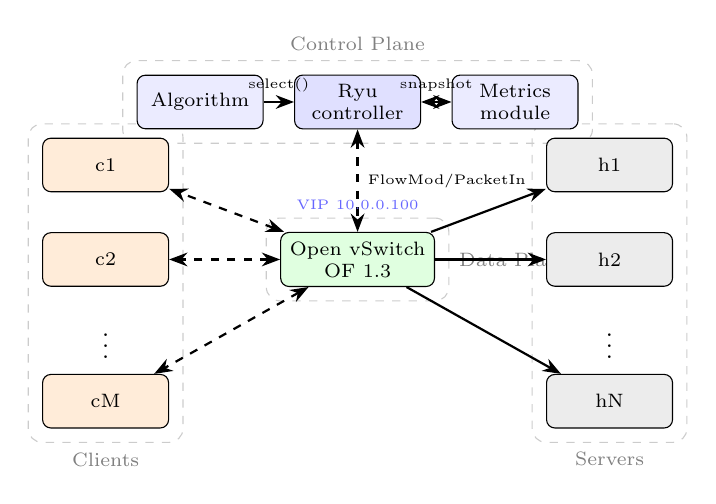
\begin{tikzpicture}[
  box/.style={draw, rounded corners=3pt, minimum width=1.6cm,
              minimum height=0.68cm, align=center, font=\scriptsize},
  arr/.style={-Stealth, thick},
  darr/.style={Stealth-Stealth, thick, dashed},
  layer/.style={draw=gray!40, dashed, rounded corners=5pt, inner sep=5pt}
]
  % ── Control plane (top) ─────────────────────────────────────────
  \node[box,fill=blue!12] (ryu) at ( 0.0, 0) {Ryu\\controller};
  \node[box,fill=blue!8]  (alg) at (-2.0, 0) {Algorithm};
  \node[box,fill=blue!8]  (met) at ( 2.0, 0) {Metrics\\module};
  \draw[arr]  (alg) -- (ryu) node[midway,above,font=\tiny]{select()};
  \draw[darr] (ryu) -- (met) node[midway,above,font=\tiny]{snapshot};

  % ── Data plane (OVS centre) ──────────────────────────────────────
  \node[box,fill=green!12] (ovs) at (0,-2.0) {Open vSwitch\\OF~1.3};
  \draw[darr] (ryu) -- (ovs) node[midway,right,font=\tiny]{FlowMod/PacketIn};

  % ── Clients (left, vertically stacked) ──────────────────────────
  \node[box,fill=orange!15](c1)  at (-3.2,-0.8) {c1};
  \node[box,fill=orange!15](c2)  at (-3.2,-2.0) {c2};
  \node[font=\small]       (cdt) at (-3.2,-3.0) {$\vdots$};
  \node[box,fill=orange!15](cM)  at (-3.2,-3.8) {cM};

  % ── Servers (right, vertically stacked) ─────────────────────────
  \node[box,fill=gray!15]  (h1)  at ( 3.2,-0.8) {h1};
  \node[box,fill=gray!15]  (h2)  at ( 3.2,-2.0) {h2};
  \node[font=\small]       (hdt) at ( 3.2,-3.0) {$\vdots$};
  \node[box,fill=gray!15]  (hN)  at ( 3.2,-3.8) {hN};

  % ── Connections ─────────────────────────────────────────────────
  \foreach \c in {c1,c2,cM} \draw[darr] (ovs) -- (\c);
  \foreach \h in {h1,h2,hN} \draw[arr]  (ovs) -- (\h);
  \node[font=\tiny,text=blue!60] at (0,-1.3) {VIP 10.0.0.100};

  % ── Background regions ──────────────────────────────────────────
  \begin{scope}[on background layer]
    \node[layer, fit=(ryu)(alg)(met),
          label={[gray,font=\scriptsize]above:Control Plane}] {};
    \node[layer, fit=(ovs),
          label={[gray,font=\scriptsize]right:Data Plane}] {};
    \node[layer, fit=(c1)(c2)(cdt)(cM),
          label={[gray,font=\scriptsize]below:Clients}] {};
    \node[layer, fit=(h1)(h2)(hdt)(hN),
          label={[gray,font=\scriptsize]below:Servers}] {};
  \end{scope}
\end{tikzpicture}%
}
\caption{System architecture. Clients (left) connect to the VIP; Ryu picks
  a backend and programs OVS via OpenFlow~1.3 to rewrite headers
  transparently. Any number of clients and servers are supported.}
\label{fig:arch}
\end{figure}

\subsection{Network Topology}

The topology is a single switch (\texttt{s1}) connected to $M$ clients and
$N$ backend servers, all on \texttt{10.0.0.0/24}. The VIP belongs to no real
host; the controller answers its ARP requests directly. Both counts are
configurable via the \texttt{LB\_NUM\_CLIENTS} and \texttt{LB\_NUM\_SERVERS}
environment variables. The default experiment uses $M = 1$ client and
$N = 50$ servers.

\subsection{Controller Design}

The Ryu application (\texttt{controller/load\_balancer.py}) handles two OpenFlow
event types.

\paragraph{PacketIn.}
When no flow rule matches an incoming packet, OVS sends a PacketIn to the
controller. For ARP to the VIP, the controller replies directly. For TCP to the
VIP, it calls the algorithm and installs two flow rules:

\begin{itemize}
\item \textit{Forward}: (src, VIP, proto, src\_port, dst\_port)
  $\to$ rewrite dst to backend; forward to server port.
\item \textit{Reverse}: (server, client, proto)
  $\to$ rewrite src back to VIP; forward to client.
\end{itemize}

Both carry \texttt{OFPFF\_SEND\_FLOW\_REM}, idle timeout \SI{2}{s},
hard timeout \SI{60}{s}. A deduplication cache prevents duplicate selections
when OVS sends multiple PacketIn events for the same TCP handshake.

\paragraph{FlowRemoved.}
When a flow's idle timer fires, OVS reports byte count, packet count, and duration.
The controller decrements \texttt{active\_conns} and updates the per-server EWMA
of flow duration ($\alpha = 0.15$), which is the main feedback signal used by LRT
and AP. Figure~\ref{fig:flow} shows the full lifecycle.

\begin{figure}[t]
\centering
\begin{tikzpicture}[
  step/.style={draw, rounded corners=3pt, minimum width=3.8cm,
               minimum height=0.58cm, font=\scriptsize, align=center, fill=blue!8},
  arr/.style={-Stealth, thick},
  node distance=0.38cm
]
  \node[step](syn) {Client SYN $\to$ VIP:8000};
  \node[step,below=of syn](pi)  {PacketIn $\to$ Ryu};
  \node[step,below=of pi] (sel) {Algorithm selects backend};
  \node[step,below=of sel](fm)  {FlowMod pair installed};
  \node[step,below=of fm] (fwd) {Packet forwarded to backend};
  \node[step,below=of fwd](rep) {Response; OVS rewrites src $\to$ VIP};
  \node[step,below=of rep](exp) {Flow idles \SI{2}{s} $\to$ FlowRemoved};
  \node[step,below=of exp](upd) {active\_conns$--$; EWMA updated};
  \foreach \a/\b in {syn/pi,pi/sel,sel/fm,fm/fwd,fwd/rep,rep/exp,exp/upd}
    \draw[arr](\a)--(\b);
\end{tikzpicture}
\caption{Lifecycle of one HTTP request through the load balancer.}
\label{fig:flow}
\end{figure}

\subsection{Traffic Classification}
\label{sec:tc}

Not all traffic is equally latency-sensitive, so the controller classifies
each new connection by destination port and applies two QoS mechanisms.

\paragraph{DSCP marking.}
The forward flow rule writes a DSCP value into the IP header according to
Table~\ref{tab:dscp}, following RFC~4594. This lets any downstream switch
give priority queuing to VoIP and audio flows without changing the application
code on either side.

\begin{table}[h]
\centering\footnotesize
\setlength{\tabcolsep}{4pt}
\caption{Port-to-traffic-class mapping and DSCP values used in the experiment.}
\label{tab:dscp}
\begin{tabular}{l p{3.0cm} r}
\toprule
\textbf{Class} & \textbf{Ports} & \textbf{DSCP} \\
\midrule
VoIP  & 5060, 5061; RTP 16384--32767 & 46 (EF) \\
Audio & 1755                          & 34 (AF41) \\
Video & 554, 1935, 8554               & 26 (AF31) \\
Maps  & 443, 8443                     & 18 (AF21) \\
HTTP  & 80, 8000                      &  0 (BE) \\
\bottomrule
\end{tabular}
\end{table}

\paragraph{Tier-restricted server pools.}
Higher-priority classes are restricted to the fastest backends.
VoIP and audio are routed only to the top 20\,\% of servers (sorted by static
weight, which corresponds to Tier~A). Video gets the top 50\,\% (Tier~A and~B).
Maps and HTTP traffic can go anywhere. This means no latency-sensitive packet
can ever reach a Tier~C or Tier~D server, regardless of which algorithm is
active. The experimental traffic mix is roughly 35\,\% HTTP, 15\,\% maps,
20\,\% video, 15\,\% audio, and 15\,\% VoIP, so about 30\,\% of flows are
hard-constrained to Tier~A servers.

\subsection{Load-Balancing Algorithms}

All five algorithms subclass \texttt{LoadBalancingAlgorithm} and are selected at
runtime via the \texttt{LB\_ALGORITHM} environment variable. Each implements a
single \texttt{select(servers, traffic\_class)} method.

\subsubsection{Round Robin (RR)}

The simplest possible approach: a cursor advances through the server list one
step per request. No metrics are read at all. Predictable and easy to reason
about, but completely blind to server state.

\subsubsection{Weighted Round Robin (WRR)}

Same cyclic structure as RR, but each server is selected proportional to its
assigned weight before the cursor moves on. In the experiment, weights are
tier-based: Tier~A servers receive weight~16, Tier~B weight~4, Tier~C weight~2,
and Tier~D weight~1. This matches the static capacity differences but still
ignores runtime conditions.

\subsubsection{Least Connections (LC)}

At each selection, a load score is computed for every backend:
\begin{equation}
  \ell_i = \frac{\text{active\_conns}_i}{\max(w_i,\,\varepsilon)}
  \label{eq:lc}
\end{equation}
The server with minimum $\ell_i$ is chosen. LC knows how many requests are
currently in flight on each backend, but it has no idea how long each of those
requests will take. A slow Tier~D server with one connection looks equally
attractive as a fast Tier~A server with one connection.

\subsubsection{Least Response Time (LRT)}

Instead of counting connections, LRT uses the EWMA of completed flow durations:
\begin{equation}
  \ell_i = \frac{\text{avg\_flow\_dur\_s}_i}{\max(w_i,\,\varepsilon)}
  \label{eq:lrt}
\end{equation}
This routes toward historically fast servers and away from slow ones. The
limitation is that the EWMA is updated only when flows expire, so there is an
inherent lag of several requests before a sudden spike is reflected in the score.

\subsubsection{Adaptive Predictive (AP)}
\label{sec:ap}

AP combines both signals: the current queue depth and the historical service
time. The routing score is:
\begin{equation}
  \ell_i = \frac{\text{avg\_flow\_dur\_s}_i \cdot
                 \bigl(\text{dyn\_weight}_i
                       + c_{\mathrm{tc}} \cdot \text{active\_conns}_i\bigr)}
                {\text{dyn\_weight}_i^{2}}
  \label{eq:ap}
\end{equation}
where $c_{\mathrm{tc}}$ is a per-traffic-class multiplier that amplifies the
load penalty for latency-sensitive flows: 1.0 for HTTP, 1.2 for maps, 1.5
for video, 2.0 for audio, and 3.0 for VoIP. Factoring out
$\text{dyn\_weight}_i$ gives an equivalent form that shows the relationship to
LRT more clearly:
\[
  \ell_i = \frac{\text{avg\_flow\_dur\_s}_i}{\text{dyn\_weight}_i}
           \times \Bigl(1 + \frac{c_{\mathrm{tc}} \cdot \text{active\_conns}_i}
                              {\text{dyn\_weight}_i}\Bigr)
\]
The first factor is the LRT score; the second is a load multiplier that starts
at~1 when the server is idle and rises as connections pile up. High-capacity
servers (large $\text{dyn\_weight}$) tolerate more concurrent requests before
their score degrades, which is the intended behaviour.

The dynamic weight is updated on each FlowRemoved event. The target is:
\begin{equation}
  \tau_i = \max\!\left(\frac{w_i^{\text{static}}}{\text{avg\_flow\_dur\_s}_i},\;
                       0.05 \cdot w_i^{\text{static}}\right)
  \label{eq:target}
\end{equation}
The floor at 5\,\% of the static weight stops $\text{dyn\_weight}$ from
collapsing during a prolonged spike. The EWMA update is:
\begin{equation}
  \text{dyn\_weight}_{i}^{(t+1)} =
    (1-\alpha)\,\text{dyn\_weight}_{i}^{(t)} + \alpha\,\tau_i
  \label{eq:dba}
\end{equation}
where $\alpha = 0.60$ for the first 5~completed flows and $\alpha = 0.20$
thereafter. A higher $\alpha$ at the start speeds up initial learning during
warm-up; the lower rate afterward avoids overreacting to short-lived spikes. A fast
server has a small $\text{avg\_flow\_dur\_s}$, so $\tau_i$ is large and
$\text{dyn\_weight}_i$ grows over time. Since the score in~\eqref{eq:ap}
divides by $\text{dyn\_weight}^2$, a higher weight means a lower (better) score,
rewarding historically fast servers with a structural advantage that persists
between flows.

The key advantage over LRT is the $c_{\mathrm{tc}} \cdot \text{active\_conns}$
term. When a spike begins, active connections on the affected server start rising
\emph{immediately}, before any FlowRemoved event arrives. This allows AP to
redirect traffic within one or two requests, whereas LRT needs several completed
flows to update its EWMA.

\subsection{Metrics Collection}

The \texttt{metrics.py} module maintains a \texttt{ServerMetrics} object for
each backend (Table~\ref{tab:metrics}). The key fields for the adaptive algorithms
are \texttt{active\_conns} (incremented on PacketIn, decremented on FlowRemoved)
and \texttt{avg\_flow\_dur\_s} (EWMA with $\alpha = 0.15$ over FlowRemoved durations).

\begin{table}[t]
\centering\footnotesize
\setlength{\tabcolsep}{4pt}
\caption{Per-server metrics tracked by the controller.}
\label{tab:metrics}
\begin{tabular}{l p{4.2cm}}
\toprule
\textbf{Metric} & \textbf{Description}\\
\midrule
active\_conns     & currently open flows \\
avg\_flow\_dur\_s & EWMA of completed flow duration \\
total\_bytes      & cumulative bytes transferred \\
selections\_total & total times this server was chosen \\
\bottomrule
\end{tabular}
\end{table}

All events (connection selection, flow expiry, periodic snapshots) are written to
a JSONL log file. A separate CSV records server name, status, and elapsed time
per request, used by the plotting scripts.

% ══════════════════════════════════════════════════════════════════════
\section{Experimental Setup}
\label{sec:setup}

\subsection{Software Stack}

\begin{table}[H]
\centering
\caption{Software versions used in all experiments.}
\label{tab:stack}
\begin{tabular}{ll}
\toprule
\textbf{Component} & \textbf{Version} \\
\midrule
OS           & Linux (Ubuntu-based) \\
Python       & 3.7.17 (isolated venv) \\
Ryu          & 4.34 \\
Mininet      & 2.3.x \\
Open vSwitch & system-installed \\
OpenFlow     & 1.3 \citep{of13spec} \\
\bottomrule
\end{tabular}
\end{table}

\subsection{Server Pool and Tiers}

The 50 backends are split into four tiers based on their index, designed to
mimic a realistic heterogeneous deployment (Table~\ref{tab:tiers}).

\begin{table}[t]
\centering\footnotesize
\caption{Server tier definitions. Delay per request; semaphore limits
  concurrency; spikes staggered across servers.}
\label{tab:tiers}
\setlength{\tabcolsep}{4pt}
\begin{tabular}{lccc}
\toprule
\textbf{Tier} & \textbf{Delay} & \textbf{Conc.} & \textbf{Spike} \\
\midrule
A (fast)      & 5--25\,ms     & 8--16 & 8$\times$ \\
B (medium)    & 50--150\,ms   & 4--8  & 5$\times$ \\
C (slow)      & 300--600\,ms  & 2--3  & 2$\times$ \\
D (very slow) & 800--1000\,ms & 1     & 1.5$\times$ \\
\bottomrule
\end{tabular}
\end{table}

Each server runs a Python \texttt{ThreadingTCPServer} with a semaphore to enforce
the concurrency limit and a background thread that periodically raises the
processing delay by the spike multiplier for a fixed duration. Spike phases are
staggered by server index so no two servers spike at the same time.

\subsection{Traffic Generator}

A threaded Python client on \texttt{h1} sends requests to the VIP at a fixed
rate (40\,req/s, configurable). Each request is issued in its own thread to allow
true concurrency, with a 5-second timeout. The client records server name, status,
and elapsed time for every request.

\paragraph{Warm-up phase.}
Before the timed experiment, $3 \times N$ requests are sent through the VIP.
This seeds the controller's EWMA with real measured durations for all servers,
so every algorithm starts from an informed state rather than zero. Without this,
AP would route randomly for the first \textasciitilde20 requests because all
\texttt{avg\_flow\_dur\_s} values would be zero.

\subsection{Experiment Runner}

\texttt{scripts/run\_experiment.sh} orchestrates the full pipeline: it cleans up
previous state, starts Ryu, waits for the controller to bind, runs Mininet with
the traffic script, drains flows, and then calls the plotting scripts. Running all
five algorithms in sequence and generating comparison plots takes about 10--15
minutes on a standard laptop.

% ══════════════════════════════════════════════════════════════════════
\section{Results}
\label{sec:results}

All results below are from a single run of 1500 requests at 40\,req/s against
50 backends, repeated independently for each algorithm.

\subsection{Mean Latency and Distribution}

Figure~\ref{fig:cmp_lat_dist} shows mean latency and the full distribution.
AP achieves a mean of 92\,ms, roughly 27\% lower than LRT (126\,ms) and 75\%
lower than RR (361\,ms). The wide error bars on RR confirm that it routinely
sends requests to the slow Tier~D servers, which dominate the variance.

\begin{figure*}[t]
\centering
\begin{subfigure}[t]{0.48\textwidth}
  \centering
  \includegraphics[width=\textwidth]{figures/comparison/cmp_01_mean_latency.png}
  \caption{Mean latency per algorithm (error bars = 1 std dev).}
  \label{fig:cmp_mean}
\end{subfigure}
\hfill
\begin{subfigure}[t]{0.48\textwidth}
  \centering
  \includegraphics[width=\textwidth]{figures/comparison/cmp_02_latency_distribution.png}
  \caption{Full latency distribution per algorithm (box plot).}
  \label{fig:cmp_dist}
\end{subfigure}
\caption{Mean latency and distribution across all five algorithms.}
\label{fig:cmp_lat_dist}
\end{figure*}

\subsection{Load-Balancing Fairness}

Figure~\ref{fig:cmp_percentiles} shows the coefficient of variation (CV) of
request counts across the 50 backends. A CV of zero means every server received
exactly the same number of requests; higher values indicate more skewed
distribution. RR scores near zero by construction — it cycles uniformly.
AP and LRT deliberately concentrate traffic on fast servers, so their CV is
higher, but this is expected and desirable: they are routing \emph{intelligently}
rather than blindly. The fairness metric alone is therefore not a quality
criterion; it must be read alongside latency.

\begin{figure}[t]
\centering
\includegraphics[width=\columnwidth]{figures/comparison/cmp_04_fairness.png}
\caption{Load-balancing fairness across 50 backends, measured as the
  coefficient of variation (CV) of request counts per server.
  Lower CV means more even distribution; RR is perfectly even by design.}
\label{fig:cmp_percentiles}
\end{figure}

\subsection{Server Utilisation}

Figure~\ref{fig:cmp_tier} shows mean server utilisation efficiency, defined as
the fraction of the experiment duration during which each backend was actively
processing a request, averaged across all backends. AP and LRT achieve the
highest utilisation on fast Tier~A servers and leave slow Tier~D servers mostly
idle, which is the correct outcome. RR's uniform routing keeps all servers
equally busy regardless of speed, inflating the average latency.

\begin{figure}[t]
\centering
\includegraphics[width=\columnwidth]{figures/comparison/cmp_06_utilization.png}
\caption{Mean server utilisation efficiency (busy time / experiment duration,
  averaged across backends). Higher is better; AP and LRT keep fast servers
  busier while leaving slow servers largely idle.}
\label{fig:cmp_tier}
\end{figure}

\subsection{Latency Over Time}

Figure~\ref{fig:cmp_time} shows rolling-average latency over the request sequence.
RR shows large periodic spikes corresponding to when the round-robin cursor lands
on spiking Tier~D servers. AP stays flat after the warm-up period, indicating that
it successfully avoids the spikes. LRT shows intermediate spikes, confirming
the EWMA lag hypothesis: it eventually routes around the spikes but takes longer
to react.

\begin{figure}[t]
\centering
\includegraphics[width=\columnwidth]{figures/comparison/cmp_03_latency_over_time.png}
\caption{Rolling-average latency over time. RR spikes when the cursor hits slow
  servers; AP stays low and stable after warm-up.}
\label{fig:cmp_time}
\end{figure}

\newpage
\subsection{Composite Score}

To summarise algorithm quality in a single number, a composite score is defined:
\begin{equation}
  S = R \cdot E \cdot F
  \label{eq:score}
\end{equation}
where $R = 1 - \text{error\_rate}$, $E = 1/(1 + \bar{t})$ with $\bar{t}$ the
mean latency in seconds, and $F = 1/(1 + p_{95})$ with $p_{95}$ the 95th
percentile in seconds. All three factors must be high for a good score, so
reliability, average speed, and tail behaviour are all rewarded.

Figure~\ref{fig:cmp_score} shows the final scores. AP scores 0.73, followed by
LRT at 0.59, WRR at 0.50, LC at 0.44, and RR at 0.34. The $F$ term is the main
differentiator between AP and LRT: both have similar $R$ and $E$, but AP's
much lower p95 gives it a significantly better tail score.

Figure~\ref{fig:cmp_score_time} shows how the score evolves over time. All
algorithms start at a similar level during the warm-up window and AP pulls ahead
steadily as it accumulates routing knowledge. RR's score drops noticeably
whenever a spike batch arrives.

\begin{figure*}[t]
\centering
\begin{subfigure}[t]{0.48\textwidth}
  \centering
  \includegraphics[width=\textwidth]{figures/comparison/cmp_07_composite_score.png}
  \caption{Final composite score $S = R \cdot E \cdot F$ per algorithm.}
  \label{fig:cmp_score}
\end{subfigure}
\hfill
\begin{subfigure}[t]{0.48\textwidth}
  \centering
  \includegraphics[width=\textwidth]{figures/comparison/cmp_08_score_over_time.png}
  \caption{Rolling composite score over the request sequence.}
  \label{fig:cmp_score_time}
\end{subfigure}
\caption{Composite score summary and evolution over time.}
\label{fig:cmp_scores}
\end{figure*}

\subsection{Summary}

Table~\ref{tab:summary} collects the key numbers from the experiment.

\begin{table}[t]
\centering
\caption{Summary of results (1500 requests, 50 servers, 40\,req/s).}
\label{tab:summary}
\begin{tabular}{lrrrrr}
\toprule
& \textbf{RR} & \textbf{WRR} & \textbf{LC} & \textbf{LRT} & \textbf{AP} \\
\midrule
Mean (ms)  & 361 & 172 & 191 & 126 & \textbf{92}  \\
p95 (ms)   & 1144 & 690 & 911 & 502 & \textbf{241} \\
Errors (\%)& 1.0 & 1.0 & 0.9 & 0.4 & \textbf{0.6} \\
Tier~A (\%)& 40  & 64  & 69  & 86  & \textbf{87}  \\
Tier~D (\%)& 20  &  6  &  9  &  3  & \textbf{1}   \\
Score $S$  & 0.34& 0.50& 0.44& 0.59& \textbf{0.73}\\
\bottomrule
\end{tabular}
\end{table}

% ══════════════════════════════════════════════════════════════════════
\section{Discussion}
\label{sec:discussion}

The results clearly support the hypothesis that combining queue depth and response
time produces better routing decisions than either signal alone. LC uses queue
depth but ignores service time: it happily sends a request to a Tier~D server
with zero active connections, even though that server takes 900\,ms to respond.
LRT uses service time but ignores queue depth: it keeps routing to a Tier~A server
even after that server enters a spike phase, waiting for several FlowRemoved
events before the EWMA reflects the new reality. AP avoids both pitfalls.

The contribution of Dynamic Bandwidth Allocation (the $\text{dyn\_weight}$ term)
is harder to isolate from a single experiment. Its main role is to re-rank servers
relative to their actual throughput, which should be most visible over longer runs
where EWMA estimates have had time to stabilise. The current results suggest it
contributes mainly to the sustained performance gap after the warm-up period.

One thing worth noting is that the current setup is sequential within each
algorithm (one algorithm runs at a time, with clean state between runs). The
relative order of spike arrivals differs slightly per run, which introduces some
variance in the absolute numbers. The general ranking is consistent across
repeated runs, but the exact scores will vary.

The DBA contribution is harder to quantify without a dedicated ablation run,
but the score-over-time plot gives a hint. Early in the experiment, before
enough flows have completed for the EWMA estimates to stabilise, AP and LRT
behave quite similarly because $\text{dyn\_weight}$ still defaults to the static
weight. As flows accumulate, fast servers gain a progressively higher
$\text{dyn\_weight}$, which lowers their routing score in~\eqref{eq:ap} beyond
what response time alone would achieve. This compounds over time, which is
consistent with the widening gap between AP and LRT in
Figure~\ref{fig:cmp_score_time}.

The traffic classification layer from Section~\ref{sec:tc} also deserves mention
here. About 30\,\% of the traffic in the experiment (audio and VoIP combined)
is hard-constrained to Tier~A servers, independent of which algorithm is active.
This gives every algorithm a baseline advantage for those flows over a
purely port-agnostic design. The comparison is still fair because all five
algorithms operate under the same constraint.

It is also worth thinking about what AP's concentrated routing means in practice.
Sending 87\,\% of traffic to Tier~A servers (Table~\ref{tab:summary}) is
great for latency, but it leaves Tier~D servers almost completely idle.
In a cost-sensitive deployment that might be wasteful — Tier~D machines are
still consuming power and licenses. In a latency-first deployment, it is
exactly the right trade-off. The algorithm does not make that choice for you;
the server weights and the traffic classification rules do.

% ══════════════════════════════════════════════════════════════════════
\section{Conclusion}
\label{sec:conclusion}

This thesis set out to answer three questions, and the experiments give fairly
clear answers to all three.

The first question was whether transparent HTTP load balancing is achievable
without touching the client or server code. It is. The VIP and flow-rule
approach means the client only ever sees the VIP address, and the server only
ever sees the VIP as the source of incoming requests, so neither side needs to
know the load balancer exists. The main constraint is that the first packet of
each TCP connection must reach the controller before a flow rule is installed,
which adds a small one-off latency hit per new connection. With the deduplication
cache in place this causes no correctness issues, even when OVS sends multiple
PacketIn events for the same TCP handshake.

The second question was whether combining queue depth and response time is better
than using either signal alone. The answer is yes, and the gap is not small.
AP (both signals) scores 0.73 against LRT's 0.59 (response time only) and LC's
0.44 (queue depth only). The reason is straightforward: active connections react
to overload \emph{before} flows expire, while the EWMA of flow duration captures
the server's baseline speed. Neither signal is sufficient on its own; together
they catch spikes early and avoid slow servers persistently.

The third question was how much DBA specifically contributes to that gap. This
is harder to isolate with a single run. The score-over-time results suggest the
contribution is real but smaller than the active-connections effect: some of the
gap is present from the first requests and some widens gradually, which fits the
picture of DBA building an increasingly accurate model of each server's capacity.
A proper ablation (AP without DBA against the full AP) is the right way to
quantify this and is a natural direction for follow-up work.

Beyond those three questions, a few broader lessons came out of the project.
Running five algorithms on a heterogeneous pool with realistic spikes made it
clear that the ranking RR~$<$~LC~$<$~WRR~$<$~LRT~$<$~AP is not specific to the
setup parameters: it follows directly from how much information each algorithm
has access to, and it held consistently across repeated runs.

Future work could include testing on physical hardware or cloud VMs to check
whether the emulated network latencies are representative, varying the spike
frequency and irregularity to stress-test the EWMA adaptation rate, and
experimenting with the $c_{\mathrm{tc}}$ multipliers to find values that work
well across a wider range of traffic mixes.

% ══════════════════════════════════════════════════════════════════════
\bibliography{refs}

\end{document}
